\documentclass[12pt]{article}
\usepackage{amsmath}
\usepackage{amssymb}
\usepackage{listings}
\usepackage{hyperref}
\usepackage{appendix}
\usepackage{graphicx}
\usepackage[margin=1in]{geometry}

\lstset{
language=C,
basicstyle=\small\sffamily,
numbers=left,
numberstyle=\tiny,
frame=tb,
columns=fullflexible,
showstringspaces=false
}

\title{\vspace{-1cm}Sparse Matrix Representation Using Finite State Transducers}
\author{\vspace{-1cm}Julian Knodt\thanks{Work done for COS 598D Systems and Machine Learning, taught by Professor Kai Li}}

\setlength{\parskip}{\baselineskip}
\begin{document}

\maketitle

\begin{abstract}
Sparse matrices are crucial for efficient operation in many different contexts which lead to
dense operations such as in pruned neural nets or in sparse graph operations. Currently, there
exist many different formats for sparse matrices, differing in efficiency of matrix operations
and compression. Most popular among representations for unstructured sparse matrices are
Compressed Sparse Row (CSR), Coordinate Order (COO), and Compressed Sparse Column (CSC). We explore
an alternative unstructured sparse matrix format, based on a data structure commonly used in
string processing: finite state transducers. We find that the proposed structure can be within
an order of magnitude of efficiency on sparse matrix vector multiplication as compared to the
CSR format, and achieves equivalent compression size. In addition, for sparsity above 0.005,
finite state transducers achieve better compression than CSR, and at all sparsity levels maintain
consistent compression rates in higher dimensions.
\end{abstract}

\section{Introduction}
Dense matrices in general provide a continuous map of indices to values. Continuous, in this
case means that every index has a corresponding well-defined value. This is costly when the matrix has a
lot of redundancy, specifically if a lot of elements are $0$. Sparse matrix formats remove the assumption
of continuity in order to improve compression, and allow for faster iteration over non-zero
elements. The utilization of sparsity is harder to optimize for than it may appear as a lot of
performance gain for matrix operations is due to the easy parallelizability of elements for use
in CPU SIMD operations or on GPUs, both of which are readily available in a dense matrix
format. Yet, there are many applications in which sparse matrices naturally arise such as
neural nets or social connection graphs, and the cost of representing them as dense matrices
becomes increasingly costly. Sparse matrices thus become essential to feasibility and efficiency
of many applications. There has been recent interest into the investigation of alternatives to
the CSR format, such as the CSR5\cite{csr5} format which optimizes the CSR format explicitly for
SIMD and GPU operations. We choose to investigate alternative storage structure, not
specifically optimizing for modern architecture. Such combinations could be investigated in
combination with the current work.

\section{Approach}

Sparse matrices's API is much closer to that of an ordered map, in that most operations
such as sparse vector-multiplication rely on efficient ordered iteration over the elements, and
random access of elements might become more costly. CSR offers an extremely efficient way to
perform iteration by representing rows implicitly as a series of pointers into column indices.
While this approach works well for 2-dimensional tensors, generalizing it requires
re-implementing it with another level of indirection, and it would not be immediately compatible
with lower dimensional tensors. A more general sparse tensor representation should be able to
generalize to higher dimensional tensors without reimplementation, ideally without loss of
efficiency.

Traditionally, an ordered map might be represented by a binary tree key-value store. but this
assumes keys and doesn't remove a ton of repetition. An alternate ordered map format is the
\textit{Finite State Transducer} (FST), used for efficient prefix and suffix compression when
storing a lot of strings. Consider indices into a matrix as strings, then it seems natural to
use finite state transducers as a way to encode sparse matrices. Notably, they present extremely
efficient compaction of large sets of strings, while having little overhead for having a diverse
set of strings with little overlap. Memory efficiency, while not directly correlated to speed,
tends to lend itself to fast iteration.

Some notable differences between a general finite state transducer and one used to encode a
matrix is that for a matrix every key's length is fixed and known ahead of time, thus we can
remove some of the dynamic elements in an FST such as checking whether a specific character is
the end of a string or not. In addition, we seek to optimize iteration efficiency, whereas most
FST's might look to optimize for flexibility of key search.

We look to match the efficacy of CSR matrix-vector multiplication and matrix-matrix
multiplication, but allow for easy representation of higher dimensional matrices.

\subsection{Finite State Transducers}

The basis for this work is the FST data structure, so we provide a short description for those
unfamiliar\footnote{For a more complete description, the
\href{https://en.wikipedia.org/wiki/Finite-state_transducer}{Wikipedia article} is more
complete, and there are many useful results from universities.}. Finite state transducers are
directed, acyclic state machines, with associated output values captured in the transition
between states. It compresses prefixes like a trie but requires that keys be added in
lexicoographic order. Essentially, they function as highly compressed ordered
maps between an input alphabet sequence and an output type. Usually, we expect variable sized
input sequences, and depending on how we might choose to encode the output type there are
necessary constraints on additive identities for the output type.

\section{Implementation}

We look at a CPU implementation of a finite state transducer with manual memory management for
maximal control over efficiency. We modify an existing FST
library\cite{FSTBlog}\footnote{Source code can be found
at\url{https://github.com/BurntSushi/fst/tree/master}. The citation references a blog that
explains the structure of the library.} and extend it to support arbitrary element types, as well
as multiple different length input encodings (byte, short, int), and other modifications.

In order to have some comparison, we implement a straight-forward CSR format. Notably, both the
FST-backed and the CSR-backed versions do not have
BLAS optimizations\footnote{For a more efficient BLAS implementation, see
\href{https://software.intel.com/en-us/mkl-developer-reference-c-sparse-blas-csr-matrix-storage-format}
{Intel's implementation}.}. We choose not to compare to a BLAS implementation, as it would take
significant engineering effort to implement something at the same level of efficiency. In general,
we expect the time complexity to be the same, but there to be a constant factor increase.
Therefore, the relative efficiency is an accurate measure of how an efficient variation of our
proposed idea would compare our implementation to an efficient CSR implementation.

Herein, we describe the major modifications made to an existing FST library, which primarily consist of
reduction of complexity, denoting contiguous ranges of elements, and creating multiple iteration
strategies.

\subsection{Reducing Complexity in the FST Library}

Due to differing desires for a general purpose FST library and one designed for matrices,
different trade-offs must be made in the underlying design. Specifically, additional costs at
run-time might be acceptable if that leads to an improvement of the compression ratio. In our case,
that trade-off is inverted, where lower run-time at the cost of increased efficiency is an
acceptable trade-off. Due to that swapped expectation, we make some notable changes to the
underlying library.

\subsubsection{Compile-time Fixed Sized Sequences}
General FST data structures allow for dynamically-sized inputs. For a matrix, we know that any
input sequence is of fixed size. While this seems like a minor modification, it also reduces the
compression size because we do not need to retain information about the length of sequences.
There is also the possibility that we can represent slices of the array using shorter sequences
and quantizing slices of the array, but that was not explored.

\subsubsection{Reduced Compilation Variants}
FST libraries also utilize multiple different compression variants, but this comes at the cost
of run-time checks. Thus, it made more sense to use a single variant that lead to some
compression loss but sped up the runtime. We also found that using a single variant did not lead
to a significant compression loss.

\subsubsection{Generalized Output Types}
The FST library being looked at could only encode input bytes with a corresponding
\lstinline{unsigned long long}. Our strategy for encoding more general input types is to add
additional encoding of input size for \lstinline{unsigned bytes, shorts, and ints}. For output types, we
require that the type implement some serialization strategy, and encode all outputs in one
array. Then to encode the correlation between an input sequence and the output, we store the
index into the array as in the original library. This allows for further optimizations because
elements stored will always be contiguous. There is also the possibility that a massive
reduction in size could be made by quantizing to a small set of elements, thus reducing the need
to store a large range of pointers.

\subsection{Marking Contiguous Ranges}
Compiler vectorization optimizations that make CSR efficient utilize compile-time knowledge
about linear accesses to an array to allow for lanes in SIMD to operate over multiple pieces of
data. In order to allow our format to take advantage of SIMD optimizations and to further
compress known patterns in the data, we utilize the fact that  we store sequential pointers
inside the last node in a sequence. That is, since we're storing in lexicographic order, and we're
storing the corresponding values as we insert, the pointer into the array will be contiguous
values, so instead of storing multiple values we store the start and end of the range.
This allows the compiler to better optimize for accessing contiguous range and add SIMD
optimizations. We found this to reduce the run-time by $0.66$, and there are likely compiler
hints that could lead to an increase in run-time.

\subsection{Iteration}
Iterating over each dimension utilizes a lot of information at run-time, such as whether the
output is a range as described in the previous section, the compressed size of multiple internal
elements, and other flags. Within each iteration, we do not want to check the state of the
flags, so we implement a plethora of different strategies, per each combination of flags, so
that these flags can be checked once and then a specific strategy can be used. This lead to
performance gain in some cases, but some other cases did not need lead to gain and those cases
were added to a more generic iteration strategy.

We also look at adding a multi-threaded iteration strategy, as such a strategy is plausible for
increasing run-time efficiency. We consider this tangential to the current work as the
single-threaded efficiency is much more representative of how efficient this could be.

\section{Experiments}

All experiments were run on a machine on a Ubuntu Linux Machine, with 1 x86\_64 Intel
i7-4770 CPU @ 3.4 GHz.

We looked at matrices from
\href{https://github.com/google-research/google-research/tree/master/state_of_sparsity}{Google's
sparse matrix research}\cite{StateOfSparsity}, using absolute thresholding in order to make the matrix sparse. Then,
we stored the matrix using the CSR format and our format and compared the two's performance.

We find that for similar input sizes, the cost in number of bytes for CSR and our proposed
format are near equivalent. As demonstrated in Figure \ref{fig:sparsity}. While not showing any
significant gains over the CSR format, when looking at higher dimensional tensors we expect it
to maintain a similar level of efficiency for sparsity.

\begin{center}
\begin{figure}
  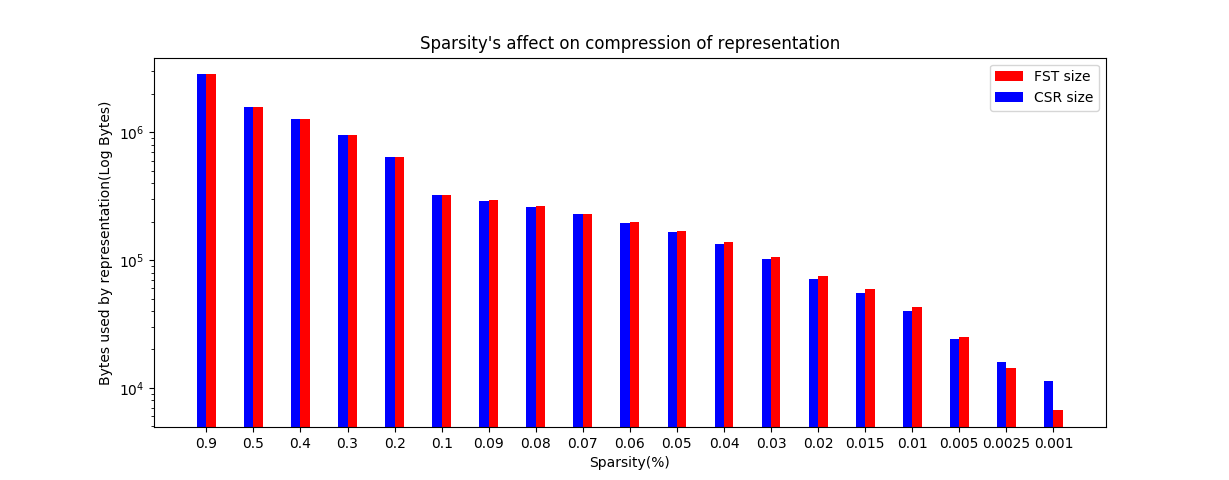
\includegraphics[width=\textwidth]{sparsity}
  \caption{The number of bytes used between a CSR format and the proposed FST format does not
differ. At extremely low sparsity, our format appears to be better, but since the overall
cost is quite small this benefit might not be significant.}
  \label{fig:sparsity}
\end{figure}
\end{center}

As shown in Figure \ref{fig:vecmul}, we find sparse vector multiplication with an FST to be an
order of  magnitude slower than the CSR implementation. We expect this to be mainly due to the fact
that CSR naturally lends itself to efficient compiler vectorization optimizations, whereas the FST-based
data structure is harder to reason about for a compiler and thus misses out on those optimizations. In
addition, due to added complexity of the storage format, there are less branches and predictions
for data prefetching than in the CSR format. With more time spent on the FST-based format using
specific knowledge of the architecture, we might expect this gap to be closed.

\begin{center}
\begin{figure}
  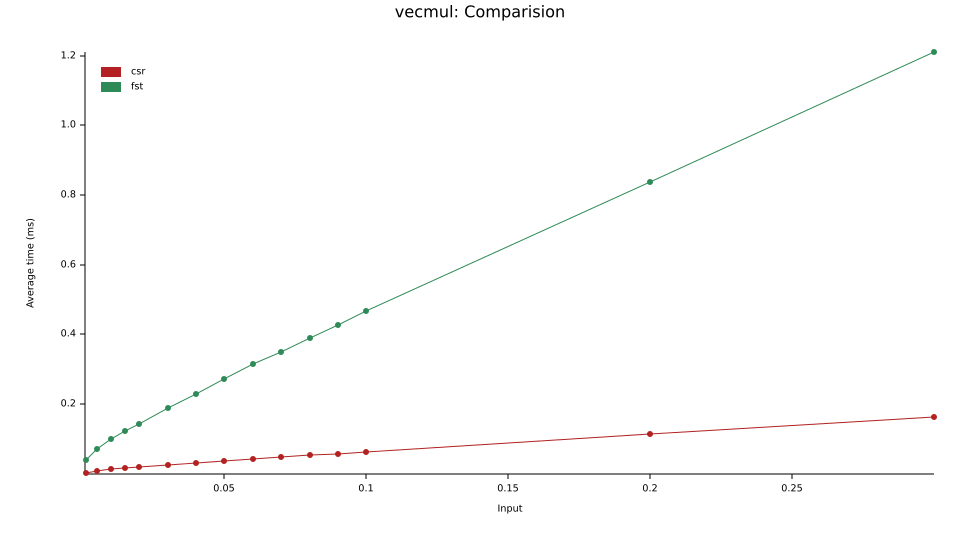
\includegraphics[width=\textwidth]{vecmul}
  \caption{The x-axis denotes the sparsity of the input matrix. The gap between the timing of the FST and the CSR formats is
  quite stark, but both lend themselves toward linear trends.}
  \label{fig:vecmul}
\end{figure}
\end{center}

We also compare the efficiency of compressing sparse matrices of similar sparsity but of
differing dimension. We generate such matrices by using an absolute threshold for elements drawn
from a random uniform distribution. Each matrix contains a total of $2^{24}$ elements. As can be
seen in Figure \ref{fig:dims}, as dimension increases there is little increase in the required number of
bytes.

\begin{center}
\begin{figure}
  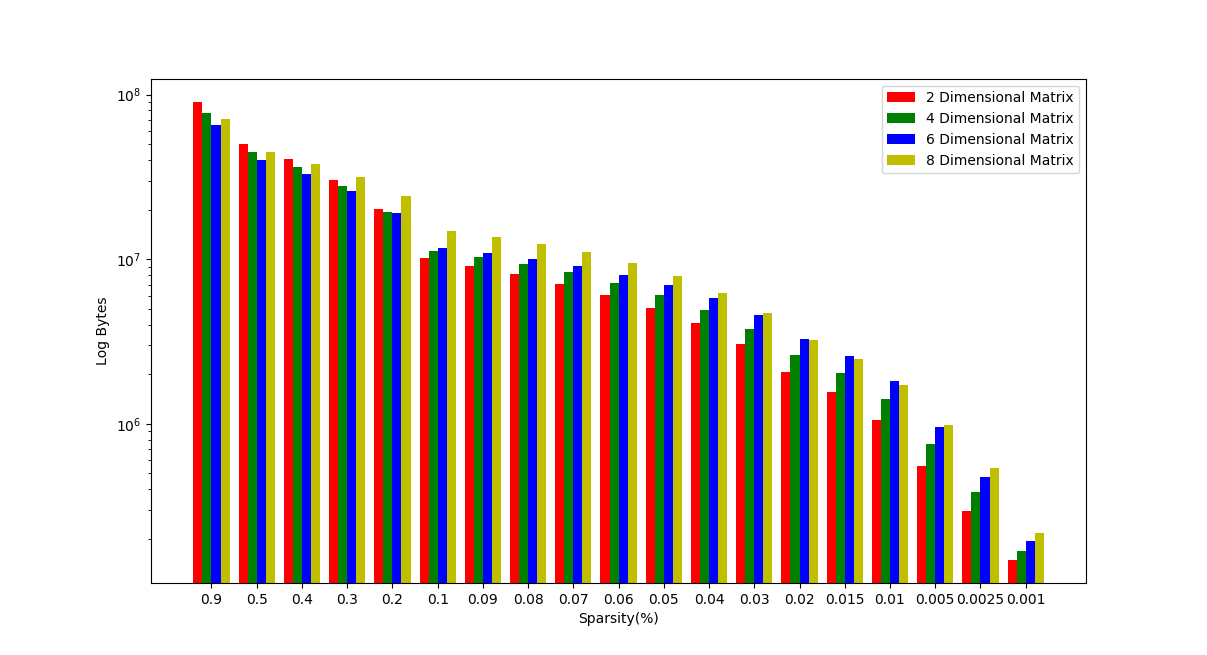
\includegraphics[width=\textwidth]{dims}
  \caption{The x-axis denotes the sparsity of the input matrix. Please note that the x-axis is
  not linear, even though it is evenly-spaced. We see that higher dimensions do   slightly correlate
  with higher number of bytes required, but not exponentially more than lower dimensions.}
  \label{fig:dims}
\end{figure}
\end{center}

A more comprehensive report of statistics gathered for vector multiplication is available
\href{https://htmlpreview.github.io/?https://raw.githubusercontent.com/JulianKnodt/mat-fst/master/reports/vecmul/report/index.html}{here}.
The benchmarks for vector multiplication are reproducible by running the benchmark in the makefile of the root directory of the
project. In order to regenerate the sparsity results, run the binaries in the
\lstinline{src/bin/} directory and the corresponding python files to create the plots.


\section*{Conclusions}
The ideas presented in this paper demonstrate an interesting approach that borrows from
studied structures in string processing. While the implementation provided does not match the
performance of the CSR format, with more engineering work we are confident the gap could be
narrowed significantly. In addition, the format provided abstracts well to higher dimensions
without loss of compression efficiency, where it may be less clear for other formats or they may
suffer large bloat in size. Our FST format provides a compromise between the CSR format and a
strided array which more easily generalizes to higher dimensions.

\subsection*{Future Work}
Most important for future directions are looking at further optimizing this library to match the
performance of the CSR format. Other interesting directions to take would be to investigate how
structured sparsity patterns affect the compression rate of the proposed format.

Apart from this, there is a lot of untested water in exploring specialized data structures from
different subfields of computer science and repurposing them, and a lot of potential exists in
doing so, as many important principles in different fields overlay the same core concepts, and
we hope this inspires further work in diversification of data structures.

\bibliographystyle{ieeetr}
\bibliography{final_report}

\newpage
\appendix
\section{Appendix}
\subsection{General Notes}
During work on this project, there were some notable realizations I came to about sparse matrix
structure.

Sparse matrices that I've looked at often do not distinguish between the indexing structure and
the elements themselves. Most of the work in sparse matrices is done on creating a structure
that specifies an efficient way to iterate through an array of elements. I have not seen a clear
distinction made between the efficiency of the indexing structure and how one can effectively
induce such a structure in a matrix. I think it might be productive to make such a distinction,
as I found it to be the case that blending iteration and indexing with the actual values in the
matrix lead to inefficiency, as one could insert the values in the matrix into the FST. In the
end, I switched to just maintaining a pointer into a contiguous array of elements and that lead
to a large performance gain because it meant in some cases I could mark elements as being ranges
over contiguous blocks, leading to efficient iteration.

I also found that the implementation we provide for FST matrices ends up looking distinctly
similar to CSR matrices but with extra adaptibility. That is, the matrix does not add any
additional overhead above the CSR format and should reduce overhead even further when rows are
missing. Thus, there really should be no performance difference between the two, as the same
amount of pointers must be followed, and the information contained is the same in between them.
This is why we expect such a format to be a good pursuit, even if the results were
disappointing.

\subsection{Convolution Algorithm with 2D Circular Buffer}
While working on this project, I realized that introducing a 2D circular buffer as an
intermediate buffer for partial sums reduces the
number of writes to the backing array. While this is not especially notable in the case of
convolving with one array, it might have some benefit when there are multiple writers, such as
when performing convolution over multiple channels in parallel to reduce memory thrashing.
This has an identical complexity to convolution which directly writes to the backing store, but
incurs an $O(K)$ memory overhead, where $K$ is the number of elements in the kernel.

\end{document}
